% !Mode:: "TeX:UTF-8"
%!TEX program  = xelatex
%“华为杯”第十八届中国研究生数学建模竞赛论文格式规范:
%论文题目和摘要写在论文摘要上,摘要页的下一页开始论文正文;
%论文从摘要页开始编写页码,页码必须位于每页页脚中部,用阿拉伯数字从“1 ”开始连续编号;
%论文题目用三号黑体字、一级标题用四号黑体字,并居中;
%论文中其他汉字一律采用小四号宋体字,行距用单倍行距。计算机结果和源程序需在规定时间内上传竞赛系统以备检查。
%请大家注意:摘要应该是一份简明扼要的详细摘要(包括关键词),请认真书写(注意篇幅一般不超过两页,且无需译成英文)。全国评阅时对摘要和论文都会审阅。
%论文不能有页眉,论文中不能有任何可能显示答题人身份的标志。
\documentclass[a4paper,10pt]{my_paper}
\usepackage{ctex}
\usepackage[top=30.0mm,bottom=25.0mm,left=22.5mm,right=22.5mm,headsep=8mm]{geometry}%设置页边距
\usepackage{array} %主要是增加列样式选项
\usepackage[dvipsnames]{xcolor}%颜色宏包
\usepackage{graphicx}%图片宏包
\usepackage{amsmath}%公式宏包
\usepackage{float} %限制浮动体的位置
\usepackage{pdfpages}
\usepackage{listings}
\usepackage{titletoc}
\usepackage{shadowtext}%大赛标题加阴影
\renewcommand{\baselinestretch}{1.0} %设置单倍行距
\graphicspath{ {./figures/} } % 插图放在这个文件夹里面
\numberwithin{equation}{section}
\usepackage{newtxtext, newtxmath}  %使用Times New Roman 字体的方法

\lstset{
    language = Python,
    backgroundcolor = \color{yellow!10},    % 背景色:淡黄
    basicstyle = \small\ttfamily,           % 基本样式 + 小号字体
    rulesepcolor= \color{gray},             % 代码块边框颜色
    breaklines = true,                  % 代码过长则换行
    %numbers = left,                     % 行号在左侧显示
    %numberstyle = \small,               % 行号字体
    keywordstyle = \color{blue},            % 关键字颜色
    commentstyle =\color{green!100},        % 注释颜色
    stringstyle = \color{red!100},          % 字符串颜色
    frame =  tb,                  % 用(带影子效果)方框框住代码块
    showspaces = false,                 % 不显示空格
    columns = fixed,                    % 字间距固定
}

%--------------------正文----------------------
\begin{document}


\numberwithin{equation}{section}
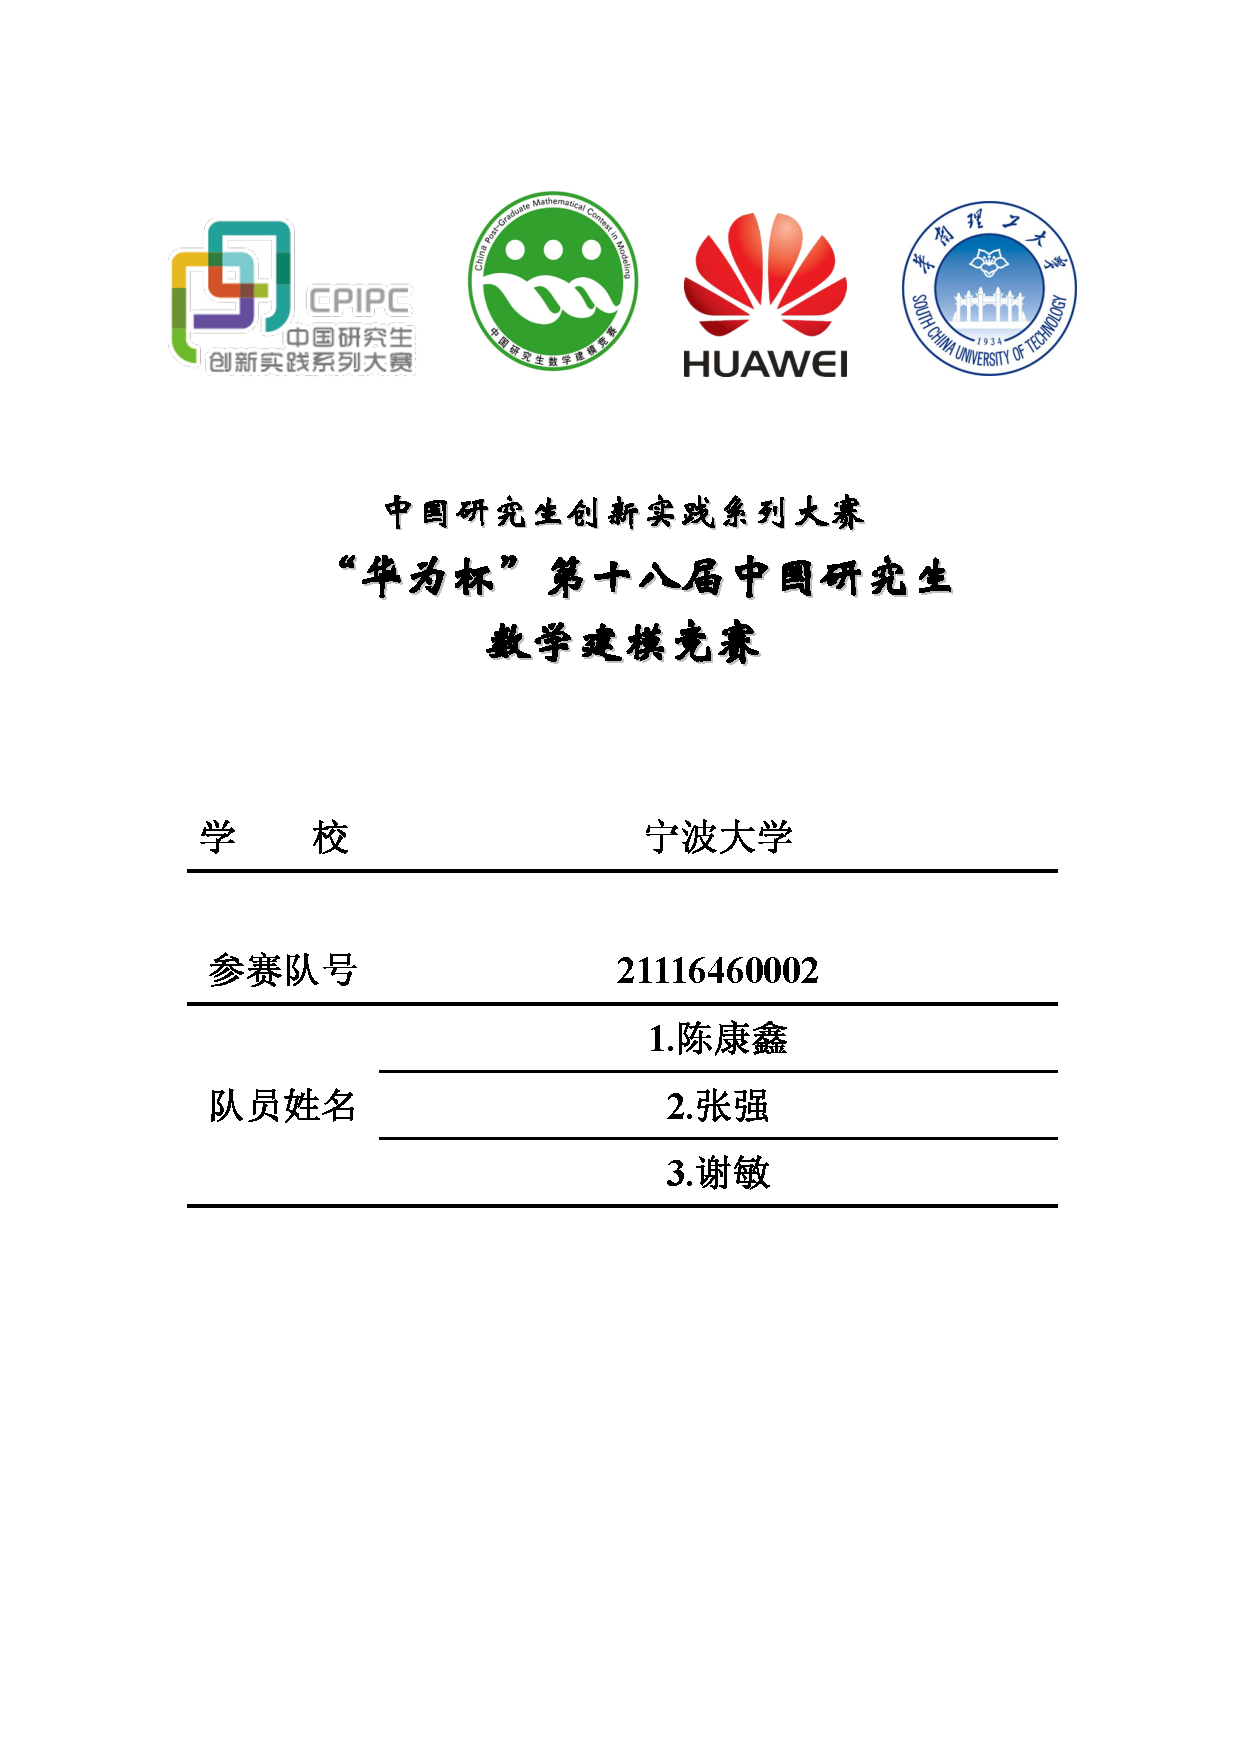
\includepdf[width=21cm]{titlepage}

%--------------------题目&摘要页----------------------
\newpage
\pagenumbering{arabic} %设置阿拉伯数字页码
\setcounter{page}{1} %正文为第一页

\begin{center}
    \zihao{-2}  \bfseries \xinwei \shadowtext{中国研究生创新实践系列大赛}

    \zihao{2} \shadowtext{\textbf{ \xinwei “华为杯”第十八届中国研究生}}

    \zihao{2} \shadowtext{\textbf{\xinwei 数学建模竞赛}}
    \end{center}

\vspace{1em}
\begin{tabular}{l p{0.8\textwidth}<{\centering}}
    \centering
    \zihao{4} 题\quad 目\quad & \zihao{3} \heiti 基于通信仿真的载波恢复算法设计与 ASIC 实现  \\ \cline{2-2}
\end{tabular}

\begin{center} \zihao{-2} \lishu 摘 \qquad 要:
\end{center}

ASIC 芯片已广泛应用于通信领域,其设计时合理平衡性能和资源,实现具体场景下
的最优设计是一项重要工作。本文从题目要求出发,使用 MATLAB 软件构建了信号传输
系统仿真框架,包括数字信号生成器、16-QAM 调制和解调、色散效应模拟与补偿、相噪
和加性高斯白噪声的模拟。在此框架上对各任务要求分别进行了算法设计与硬件实现。
%空行即换行
针对任务一,首先通过傅里叶变换分析了信道中色散效应与相位噪声的耦合机制。然
后提出了将色散效应与相位噪声去耦合的方法,即根据色散效应与相位噪声产生的时移和
频移进行补偿处理。对经过这种补偿处理后的纯净相位噪声进行了分析,提出了使用分段
线性插值算法进行相噪补偿的方法。并经推论和仿真实验验证得到在本算法的假设下采用
合适的傅里叶窗口大小,能在满足 RSNR 代价<0.3 dB 条件下使 Pilot 开销最小为 2/256。
最后进行了 ASIC 算法设计(硬件设计),根据题意给出了算法的电路结构。

针对任务二,首先确定一种导频最佳的插入方式,即首尾插入方式。然后通过 MATLAB
响应面实验工具建立色散、线宽与误码率的关系,在合理忽略色散对误码率的影响的前提
下,分析不同线宽下误码率与窗口大小的关系和固定线宽条件下窗口大小与 RSNR 代价的
关系,从而得到在设定误码率和满足 RSNR 代价<0.3 dB 条件下色散、线宽和 Pilot 开销的
关系。当线宽较大时,相噪对误码率的影响较显著,窗口大小减小有利于误码率的降低,
同时 RSNR 代价也会减小。

针对任务三,综合考虑定点量化对 CR 算法的性能和资源的影响。在任务二的基础上
首先对量化过程中产生的量化噪声进行了建模分析,得到了量化比特数和量化信噪比之间
的关系。对算法中的主要运算数据进行了数值统计用以分析量化比特数的分配。并经推论
和仿真实验验证得到在不同场景下 Polit 开销最小与芯片资源消耗相对最少的量化模型方
案。最后也进行了 ASIC 算法设计(硬件设计),根据题意给出了算法的改进电路结构,
并对整体芯片资源消耗进行了统计计算。

针对任务四,为了实现位宽自动优化并综合考虑性能和资源两种因素,考虑到资源与
芯片实现面积和功耗有关,首先建立资源使用量化评价函数。然后以 RSNR 代价作为性能
评定指标,以不同位宽向量下的 RSNR 代价与资源使用评价函数分别赋予权重因子,组成
综合评价目标函数。最后提出基于禁忌搜索算法的位宽自动优化方法,以得到性能和代价
综合评价目标函数的最优 Pareto 解集,即最优位宽设计方案。

最后本文对 CR 算法的相位噪声提取效果以及整个信号传输系统的抗噪声性能进行了
检验,检验结果为:该算法能较好地提取出信道中的相位噪声;该算法提高了整个系统的
抗噪声性能。

\vspace{1em}
\noindent \textbf{关键词:}仿真框架;CR 算法;噪声耦合;去耦合;ASIC 算法设计;量化噪声



%--------------------目录----------------------
\newpage

\begin{center}
\tableofcontents
\end{center}

%--------------------正文----------------------
%--------------------问题重述----------------------
\newpage
\section{问题重述}
\subsection{问题背景}
DSP(Digital Signal Process)即数字信号处理器,也可称为 DSP 基带芯片,它能够实
现数字信号处理技术的芯片,其特殊的 DSP 指令,可以用来快速的实现各种数字信号处理
算法[1]。这种芯片往往是基于专用集成电路(ASIC)实现的,细小的芯片具有比单光纤更
优的容量,使网络流量增长更加迅猛。ASIC 芯片算法的设计步骤如图 1.1 所示。其 DSP
算法主要分两步,首先在只考虑浮点计算的前提下根据信道损伤的物理模    型设计补偿算法;
然后根据芯片资源和功耗约束,将算法修整为 ASIC 芯片可实现的定点形式,该步骤需要
将算法细化为芯片上最基本的乘、加等运算,此外还要考虑定点量化噪声的影响。合理平 衡性能和资源,实现具体场景下的最优设计,对 DSP 芯片算法工程的应用具有重要意义。

\subsection{问题提出}
本题在不考虑色散补偿和误码率计算的复杂度和资源,只需考虑载波恢复(Carrier 
Recovery, CR)优化算法(计算相噪+补偿相噪)相关的资源的情况下,解决以下任务:

\textbf{任务一:}Pilot 开销最小的 CR 算法设计
设置波特率为 150 G baud 的标准 16QAM 信号,令线宽为 100 kHz,色散值为 20000
ps/nm,算法的并行度固定为 128,不考虑定点量化。以加法、乘法、查表和缓存为基础,
并以 RSNR 代价<0.3 dB 为目标,设计一套 Pilot 开销最小的 CR 算法。

\textbf{任务二:}色散、线宽与 Pilot 开销间的量化
设置线宽从 10 kHz~10 MHz,色散值从 0~10000 ps/nm 变化场景,以 RSNR 代价<0.3
dB 为目标,定量得到色散、线宽与 Pilot 开销的关系。

\textbf{任务三:}替换成你的内容

\textbf{任务四:}替换成你的内容
%--------------------模型假设----------------------
\section{模型假设}
1. 假设本文 CR 算法中接收端的载波已同步;

2. 假设色散补偿时不考虑定点量化的影响;

3. 假设把加入的色散当作已知进行直接补偿

%--------------------符号说明----------------------
\section{符号说明}

%使用三线表格最好~

%插入表格B站教程:https://www.bilibili.com/video/BV1p3411q7qG?spm_id_from=333.999.0.0、https://www.bilibili.com/video/BV1544y1b7dS?spm_id_from=333.999.0.0

\begin{table}[htb]
    \centering
    \begin{tabular}{p{2.0cm}<{\centering}p{9.0cm}<{\centering}p{2.0cm}<{\centering}}
 %指定单元格宽度, 并且水平居中。
    \hline
    符号 & 说明 & 单位 \\ %换行 
    \hline
    $\hat{S}$ & 接受信号 & V \\ %把你的符号写在这
    $S$ & 发送信号 & V \\ 
    $S_{16QAM}(t)$ &  经 16QAM 调制后的信号 &  V \\ 
    \hline
    \end{tabular}
\end{table}

%--------------------模型准备----------------------
%数学公式保姆级B站教程:https://www.bilibili.com/video/BV19f4y1n7ti?spm_id_from=333.999.0.0、https://www.bilibili.com/video/BV1F3411z7iD?spm_id_from=333.999.0.0
\section{模型准备}
(注意:这个部分根据自己的情况选择保留与否)

经过 16QAM 调制系统后的信号 S16QAM(t)如式 4.1 所示,式中最小幅度的信号能量 E0 为 A02T/2。若已调信号的最大幅度为 1,则 16QAM 信号星座图上信号点间的最小距离d16QAM如式 4.2 所示。\cite{ref1,ref2}

\begin{equation}
S_{16QAM}(t)=A_0 a_i\cos{\omega_0 t}+A_0 b_i\sin{\omega_0 t}=\sqrt{E_0}a_i \varphi_1(t)+\sqrt{E_0}b_i \varphi_2(t)
\end{equation}

\begin{align}
d_{16QAM}=\frac{\sqrt{2}}{L-1}=\frac{\sqrt{2}}{\sqrt{M}-1}=3\sqrt{2}
\intertext{式中:$L-QAM$ 信号比特位长;$M-QAM$ 电平数} \notag
\end{align}

%--------------------问题一的模型建立与求解----------------------

\section{问题一的模型建立与求解}
(注意:这个部分里面的标题可根据你的论文内容进行调整,我这里给的是一个通用的模版)

\subsection{问题的描述分析}

\subsection{数学模型的建立}

\subsection{模型求解和分析}

%--------------------问题二的模型建立与求解----------------------
\section{问题二的模型建立与求解}
(注意:这个部分里面的标题可根据你的论文内容进行调整,我这里给的是一个通用的模版)

\subsection{问题的描述分析}

\subsection{数学模型的建立}

\subsection{模型求解和分析}


%--------------------问题三的模型建立与求解----------------------
\section{问题三的模型建立与求解}
(注意:这个部分里面的标题可根据你的论文内容进行调整,我这里给的是一个通用的模版)
\begin{figure}[!h]
    \centering
    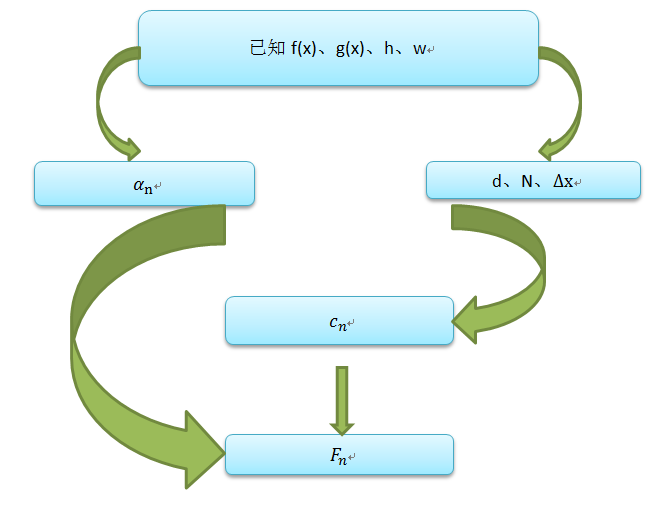
\includegraphics[width=.7\textwidth]{1.png}
    \caption{问题三流程图}
\end{figure}

\subsection{问题三分析}

\subsection{问题的描述分析}

\subsection{数学模型的建立}

\subsection{模型求解和分析}

%--------------------问题四的模型建立与求解----------------------
\section{问题四的模型建立与求解}
(注意:这个部分里面的标题可根据你的论文内容进行调整,我这里给的是一个通用的模版)

\subsection{问题的描述分析}

\subsection{数学模型的建立}

\subsection{模型求解和分析}

%--------------------模型评价----------------------
\section{模型评价}

\subsection{模型的优点}

\subsection{模型的缺点}

\subsection{模型的改进和展望}

%--------------------参考文献----------------------
%这里我使用了非bibTeX格式,B站教程:https://www.bilibili.com/video/BV1QL4y1Y7JR?spm_id_from=333.999.0.0
\addcontentsline{toc}{section}{参考文献} %将参考文献放进目录
% chenkangxin
\begin{thebibliography}{10}
\bibitem{ref1}
张雄伟. DSP 芯片的原理与开发应用[M]. 电子工业出版社, 2016.
\bibitem{ref2}
姜俊迪, 林如俭. 一种 OFDM 时域导频插入的最小二乘估计方法[J]. 电子测量技术, 2008, 31(3): 34-37.
% qiangzibro

% xiemin
\end{thebibliography}

%--------------------附录----------------------
\newpage

\appendix

\section{主程序源代码}

\begin{lstlisting}[language=Python]%设置不同语言即可。
kk=2;[mdd,ndd]=size(dd); %删除了会报错
# 问题1
print("Hello World!")
# 问题2
print("Open source is awesome!")
# 问题3
print("Open by NBU Professional Team" )
# 问题4

\end{lstlisting}


\end{document}